\documentclass[11pt,letterpaper]{article}
\usepackage[margin=0.8in]{geometry}
\usepackage[T1]{fontenc}
\usepackage{lmodern,microtype,graphicx,booktabs,amsmath,array,caption}
\usepackage[hidelinks]{hyperref}
\usepackage{fancyhdr}
\pagestyle{fancy}\fancyhf{}
\fancyhead[L]{\small COMP 664: Course Project, Fall 2026}
\fancyhead[R]{\small Topic 2}
\fancyfoot[C]{\thepage}
\setlength{\headheight}{14pt}
\setlength{\parindent}{0pt}\setlength{\parskip}{5pt}
\captionsetup{font=small,labelfont=bf,hypcap=false}
\makeatletter\let\tableinput\@@input\makeatother
\newcommand{\code}[1]{\texttt{\detokenize{#1}}}
\newcommand{\FreshOrdCleanAcc}{97.26}
\newcommand{\FreshOrdCleanAccSD}{0.16}
\newcommand{\FreshOrdCleanFone}{96.32}
\newcommand{\FreshOrdCleanFoneSD}{0.18}
\newcommand{\FreshOrdFieldAcc}{18.78}
\newcommand{\FreshOrdFieldAccSD}{1.10}
\newcommand{\FreshOrdFieldFone}{7.76}
\newcommand{\FreshOrdFieldFoneSD}{0.83}
\newcommand{\FreshAugCleanAcc}{96.66}
\newcommand{\FreshAugCleanAccSD}{0.58}
\newcommand{\FreshAugCleanFone}{95.71}
\newcommand{\FreshAugCleanFoneSD}{0.50}
\newcommand{\FreshAugFieldAcc}{20.13}
\newcommand{\FreshAugFieldAccSD}{0.74}
\newcommand{\FreshAugFieldFone}{9.16}
\newcommand{\FreshAugFieldFoneSD}{0.73}
\newcommand{\FreshDeltaAcc}{+1.35}
\newcommand{\FreshDeltaAccSD}{1.69}
\newcommand{\FreshDeltaFone}{+1.40}
\newcommand{\FreshDeltaFoneSD}{1.31}

\newcommand{\FreshConclusion}{Strong augmentation improved both field metrics on average, but the paired improvements were not consistent across all three seeds.}

\newcommand{\DemoOrdOne}{late blight}
\newcommand{\DemoAugOne}{late blight}
\newcommand{\DemoOrdTwo}{early blight}
\newcommand{\DemoAugTwo}{late blight}

\begin{document}
\begin{center}
{\Large\bfseries Plant Disease Classification Across\\Clean and Field Images}\par
\vspace{.5em}Author Name(s)\quad Fall 2026
\end{center}
\begin{abstract}
We test whether stronger crop and color augmentation improves transfer from controlled tomato-leaf photographs to field images. Building on a supplied single-seed experiment with two fixed views per image, we independently train six ImageNet-pretrained MobileNetV3-Small classifiers: ordinary and strong augmentation under three paired seeds, with fresh views sampled every epoch. The official source split and all training budgets remain fixed; checkpoint selection uses only PlantVillage validation. Ordinary training reaches $\FreshOrdCleanAcc\pm\FreshOrdCleanAccSD$\% clean accuracy and $\FreshOrdFieldAcc\pm\FreshOrdFieldAccSD$\% field accuracy. Strong augmentation reaches $\FreshAugCleanAcc\pm\FreshAugCleanAccSD$\% and $\FreshAugFieldAcc\pm\FreshAugFieldAccSD$\%, respectively (mean $\pm$ sample SD over seeds). The mean paired field changes are $\FreshDeltaAcc$ percentage points in accuracy and $\FreshDeltaFone$ in macro-F1. \FreshConclusion\ Training logs, all six checkpoints, individual predictions, independent metric audits, and an executed Notebook accompany the report.
\end{abstract}

\section{Question and comparison}
A classifier can perform well on controlled leaf photographs yet fail under different backgrounds, lighting, scales, and viewpoints. Our question is: \emph{How large is the clean-to-field gap, and can crop and color augmentation reduce it?} We use one backbone and compare two training procedures, rather than searching across architectures. Each input is one RGB photograph; the target is one of nine shared tomato labels.

The main experiment is the new three-seed, fresh-view comparison. The original two-view result is retained as a legacy reference. Fresh training uses the same examples, trainable blocks, optimizer settings, batch size, and eight-epoch budget for both conditions. All six checkpoint choices are finalized before either test set is scored.

\begin{center}
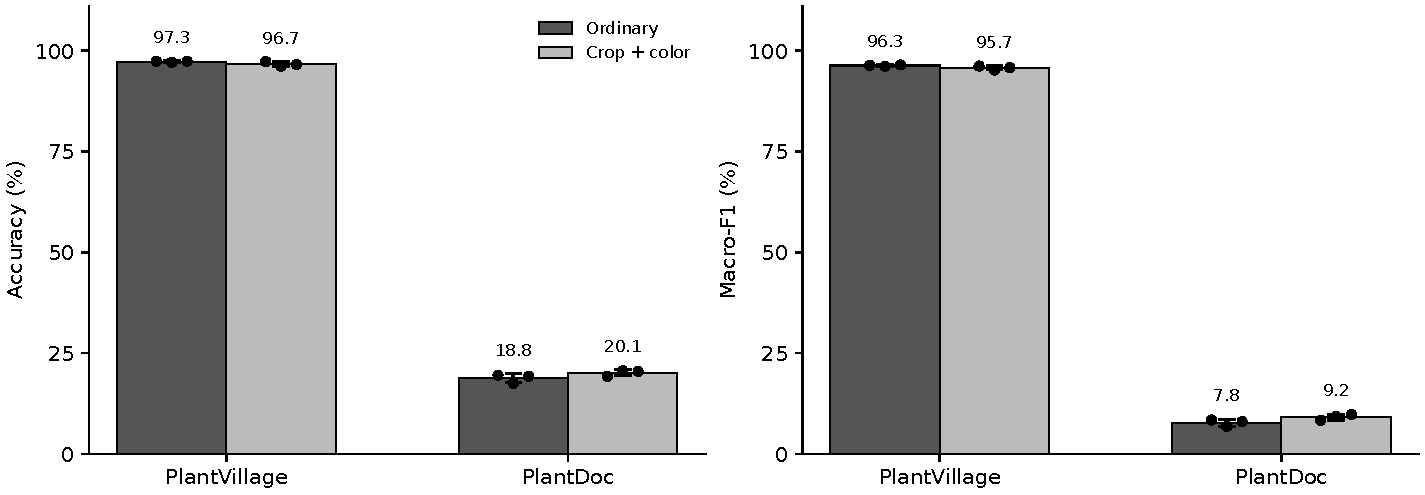
\includegraphics[width=.95\linewidth]{figures/fresh_performance.pdf}
\captionof{figure}{Fresh-view performance. Bars show the mean of three seeds; error bars show sample SD, and dots show individual runs. All runs use the same 3,351 clean and 742 field test images.}
\end{center}
\clearpage

\section{Data and split integrity}
PlantVillage provides controlled leaf photographs \cite{pv}; Cropped-PlantDoc provides the external classification images \cite{pd}. We use the nine-class mapping in the course specification and exclude PlantVillage target spot. Folder names are case-folded and stripped of non-alphanumeric characters before mapping. Exact names and class indices are saved in \code{results/class_mapping.csv}.

We preserve the official leaf-grouped PlantVillage color train/test lists. Within its original training partition, 15\% of documented leaf groups per class (rounded, split seed 664) enter validation. This data split remains identical across training seeds. Images without a documented leaf ID stay in training. PlantDoc's original train and test folders are pooled \emph{only} as the external test: no PlantDoc image enters optimization or checkpoint selection.

\begin{center}\small
\begin{tabular}{lrrrr}\toprule
Class & Train & Validation & Clean test & Field test\\\midrule
\tableinput figures/counts.tex
\midrule Total & 12,036 & 1,364 & 3,351 & 742\\\bottomrule
\end{tabular}
\captionof{table}{The original audited split, used without changes in all fresh-view runs.}
\end{center}

\textbf{Incomplete group metadata.} Exactly 4,280 training and 1,060 clean-test images lack documented leaf IDs. No retained \emph{documented} leaf group crosses splits, but unknown identities prevent a complete same-leaf independence guarantee. Mosaic virus has no documented training leaf groups and therefore zero validation examples. Selection uses the eight supported validation classes; training and both tests cover all nine. We do not create potentially leaking image-level validation samples to fill this missing class.

\textbf{Duplicate audit.} SHA-256 checks remove five source-training entries with copies in held-out splits. Among 746 mapped PlantDoc entries, two redundant same-label copies and both copies of one contradictory-label image are removed, leaving 742 byte-unique entries. These checks do not rule out visually similar crops, recompressed images, or near-duplicates. The two spider-mite examples are visually related multi-panel illustrations, so their independence and representativeness are especially uncertain.

\textbf{Reconstruction.} Fixed upstream repository revisions regenerate the original manifest, exclusions, and mapping byte for byte. During the fresh experiment, deterministic image decoding checks every loaded raw file against its recorded SHA-256. Portable disk names encode Windows-invalid characters while preserving original paths in the manifest. These are reproducibility and integrity checks, not proof that all labels are biologically correct.
\clearpage

\section{Fresh-view training protocol}
We replace the ImageNet MobileNetV3-Small output layer with nine logits \cite{mobile}. The prefix is frozen in evaluation mode; the last inverted residual block, final convolution, and classifier are trained (950,617 of 1,527,081 parameters). Within each seed, both conditions begin from the same complete state and receive exactly the same shuffled image indices in every epoch.

\begin{center}\small
\begin{tabular}{p{.27\linewidth}p{.65\linewidth}}\toprule
Setting & Prespecified value\\\midrule
Seeds and budget & 664, 665, 666; two conditions each; 8 epochs, batch 96\\
Optimization & Cross-entropy; AdamW, learning rate $5\times10^{-4}$, weight decay $10^{-4}$\\
Input and normalization & RGB, $128\times128$; ImageNet channel mean and standard deviation\\
Ordinary & Resize, horizontal flip with probability 0.5\\
Strong & Additional random crop (area .55--1.0, log-uniform aspect ratio .8--1.25); brightness/contrast/saturation jitter .35 and hue jitter .07\\
Image exposure & 12,036 images per epoch; 1,008 optimizer steps and 96,288 presentations per model\\
Selection & First epoch maximizing source-validation supported-class macro-F1\\
Execution & One RTX 5070 Ti Laptop GPU; PyTorch 2.7.1+cu128, torchvision 0.22.1+cu128; deterministic algorithms; TF32 disabled\\\bottomrule
\end{tabular}
\captionof{table}{Matched settings for the six newly trained models. No target-domain adaptation or architecture search is performed.}
\end{center}

\textbf{Fresh views, not cached random transformations.} We cache only deterministic EXIF-corrected RGB resizing as uint8 pixels. Each image receives a newly sampled PIL transformation in each epoch. A local RNG keyed by training seed, epoch, and image index makes the views reproducible independently of thread scheduling. Ordinary flip draws are fresh even though only two flipped/unflipped outcomes are possible. Strong crops and color factors are redrawn each epoch. Frozen-prefix activations are computed afresh per batch, converted to float16, then returned to float32 for the trainable blocks; they are never reused across epochs.

\textbf{Recorded evidence.} Each run logs loss, validation scores, 126 optimizer steps per epoch, sample-order hashes, initialization hashes, selected weights, and completion records. The aggregate audit checks equal initialization and order within each pair, unchanged frozen-prefix parameters, all 48 completed epochs, and a checkpoint lock written before test evaluation. Total exposure is 577,728 image presentations and 6,048 optimizer steps.

\begin{center}
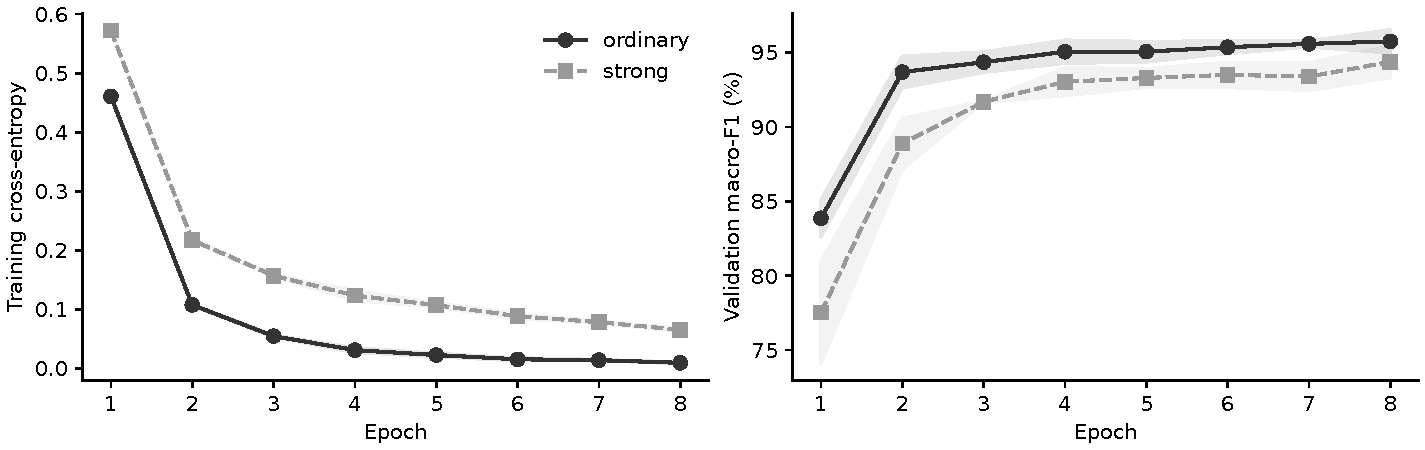
\includegraphics[width=.95\linewidth]{figures/fresh_history.pdf}
\captionof{figure}{Mean training loss and supported-class validation macro-F1 over three seeds; shading shows sample SD. Epoch selection is performed separately for each model.}
\end{center}
\clearpage

\section{Overall results and seed variability}
Accuracy is the correct-prediction fraction. Test macro-F1 averages all nine class F1 scores equally, using zero for an undefined class score. The clean-to-field gap is the clean metric minus the field metric, in percentage points (pp). A smaller gap alone does not establish improved field performance.

\begin{center}\small
\begin{tabular}{lrrrr}\toprule
 & \multicolumn{2}{c}{Accuracy (\%)} & \multicolumn{2}{c}{Macro-F1 (\%)}\\
Training & Clean & Field & Clean & Field\\\midrule
\tableinput figures/fresh_summary.tex
\bottomrule\end{tabular}
\captionof{table}{New independent training results, mean $\pm$ sample SD over the three paired seeds. These are three fits on the same test collections, not three independent datasets.}
\end{center}

\begin{center}\small
\begin{tabular}{rlrrrrr}\toprule
 & & Selected & \multicolumn{2}{c}{Accuracy (\%)} & \multicolumn{2}{c}{Macro-F1 (\%)}\\
Seed & Training & epoch & Clean & Field & Clean & Field\\\midrule
\tableinput figures/fresh_seeds.tex
\bottomrule\end{tabular}
\captionof{table}{Every run, without selection by field performance. Seed 664 is fixed as the illustrative checkpoint pair for figures and demonstrations.}
\end{center}

\begin{center}\small
\begin{tabular}{rrr}\toprule
Seed & Field accuracy change (pp) & Field macro-F1 change (pp)\\\midrule
\tableinput figures/fresh_deltas.tex
\bottomrule\end{tabular}
\captionof{table}{Paired strong-minus-ordinary changes. Their mean $\pm$ SD is $\FreshDeltaAcc\pm\FreshDeltaAccSD$ pp for accuracy and $\FreshDeltaFone\pm\FreshDeltaFoneSD$ pp for macro-F1.}
\end{center}

\FreshConclusion\ Three seeds expose training variability but remain too few for a strong claim of universal benefit or equivalence. Per-seed class-stratified paired bootstrap intervals are also supplied; they condition on each fitted pair and observed field images, and do not replace seed variability.

\textbf{Legacy reference.} The supplied two-fixed-view run achieved 97.25\% clean / 19.54\% field accuracy with ordinary training and 96.09\% / 18.73\% with strong augmentation (field macro-F1 8.67\% / 8.57\%). It used one seed, PyTorch 2.5.1 on CPU, and cached prefix activations. The new runs change view refresh, RNG implementation, streaming, and execution environment. Therefore a difference from that reference cannot be attributed purely to fresh augmentation. The controlled comparison is ordinary versus strong \emph{within} the new matched protocol.
\clearpage

\section{Per-class gaps and errors}
\begin{center}\small
\begin{tabular}{lr rrr rrr}\toprule
 & Field & \multicolumn{3}{c}{Ordinary recall (\%)} & \multicolumn{3}{c}{Strong recall (\%)}\\
Class & $n$ & Clean & Field & Gap & Clean & Field & Gap\\\midrule
\tableinput figures/fresh_recall.tex
\bottomrule\end{tabular}
\captionof{table}{Recall averaged over three seeds; gaps are differences of unrounded clean and field means in pp. Full per-seed recall/F1, SD, and class gaps are supplied as CSVs.}
\end{center}

Ordinary training most often predicted late blight, assigning that label to 540.0 of 742 field images on average (SD 85.8); its true support was 111. Strong training most often predicted late blight, assigning that label to 543.7 of 742 field images on average (SD 56.3); its true support was 111. The largest signed mean class-recall change was +10.7 pp for septoria, and the smallest was -8.3 pp for early blight.


\begin{center}
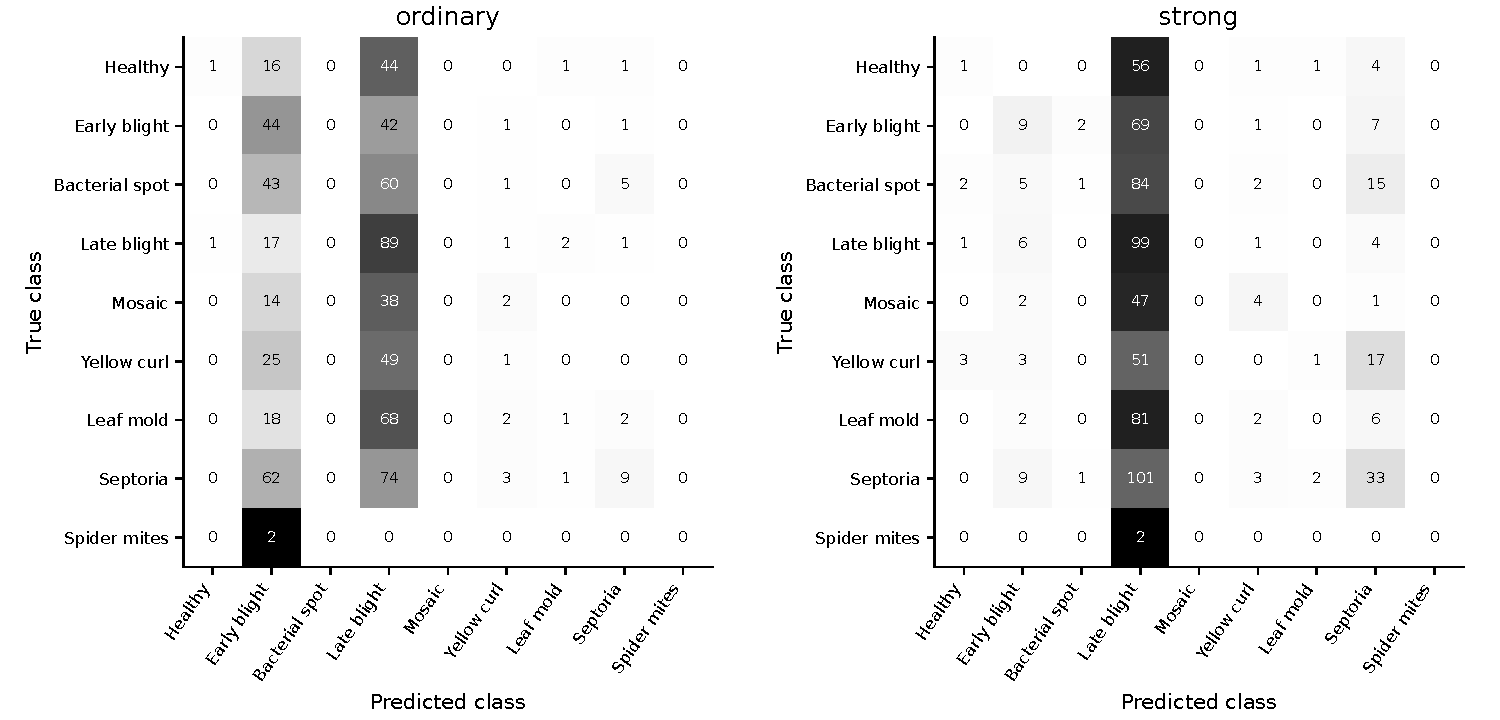
\includegraphics[width=.94\linewidth]{figures/fresh_confusions.pdf}
\captionof{figure}{Field confusion counts for the prespecified illustrative seed 664. Rows are true classes; columns are predictions. Grayscale uses the fraction within each true class. This pair was not chosen for its field score.}
\end{center}

High recall for a frequently predicted label can coexist with poor precision and zero recall for other labels. Macro-F1 exposes this concentration. The two spider-mite entries receive the same macro-F1 weight as 149 Septoria images; one changed spider-mite prediction shifts that run's class recall by 50 pp. Averaging seeds does not create additional independent spider-mite examples.
\clearpage

\section{Confidence and illustrative photographs}
\textbf{Training-only sanity baseline.} A constant classifier chosen by the most common \emph{source training} label (yellow leaf curl) achieves 32.83\% clean and 10.11\% field accuracy, with macro-F1 5.49\% and 2.04\%. No field label is used to choose this baseline. Exceeding it does not imply useful diagnostic performance.

\begin{center}\small
\begin{tabular}{rlrrr}\toprule
Seed & Training & High-confidence $n$ & Correct & Accuracy (\%)\\\midrule
\tableinput figures/fresh_confidence.tex
\bottomrule\end{tabular}
\captionof{table}{Field predictions with maximum softmax $\geq0.9$. These uncalibrated scores must not be interpreted as reliable disease probabilities.}
\end{center}

\begin{center}
\begin{minipage}{.47\linewidth}\centering
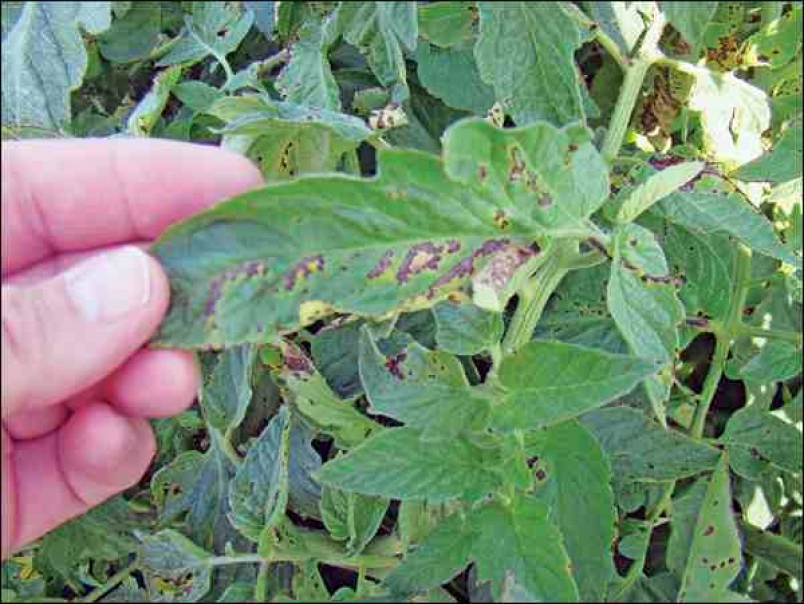
\includegraphics[height=1.8in,width=.95\linewidth,keepaspectratio]{../examples/field.jpg}\\
\small Label: early blight.\\Ordinary: \DemoOrdOne.\\Strong: \DemoAugOne.
\end{minipage}\hfill
\begin{minipage}{.47\linewidth}\centering
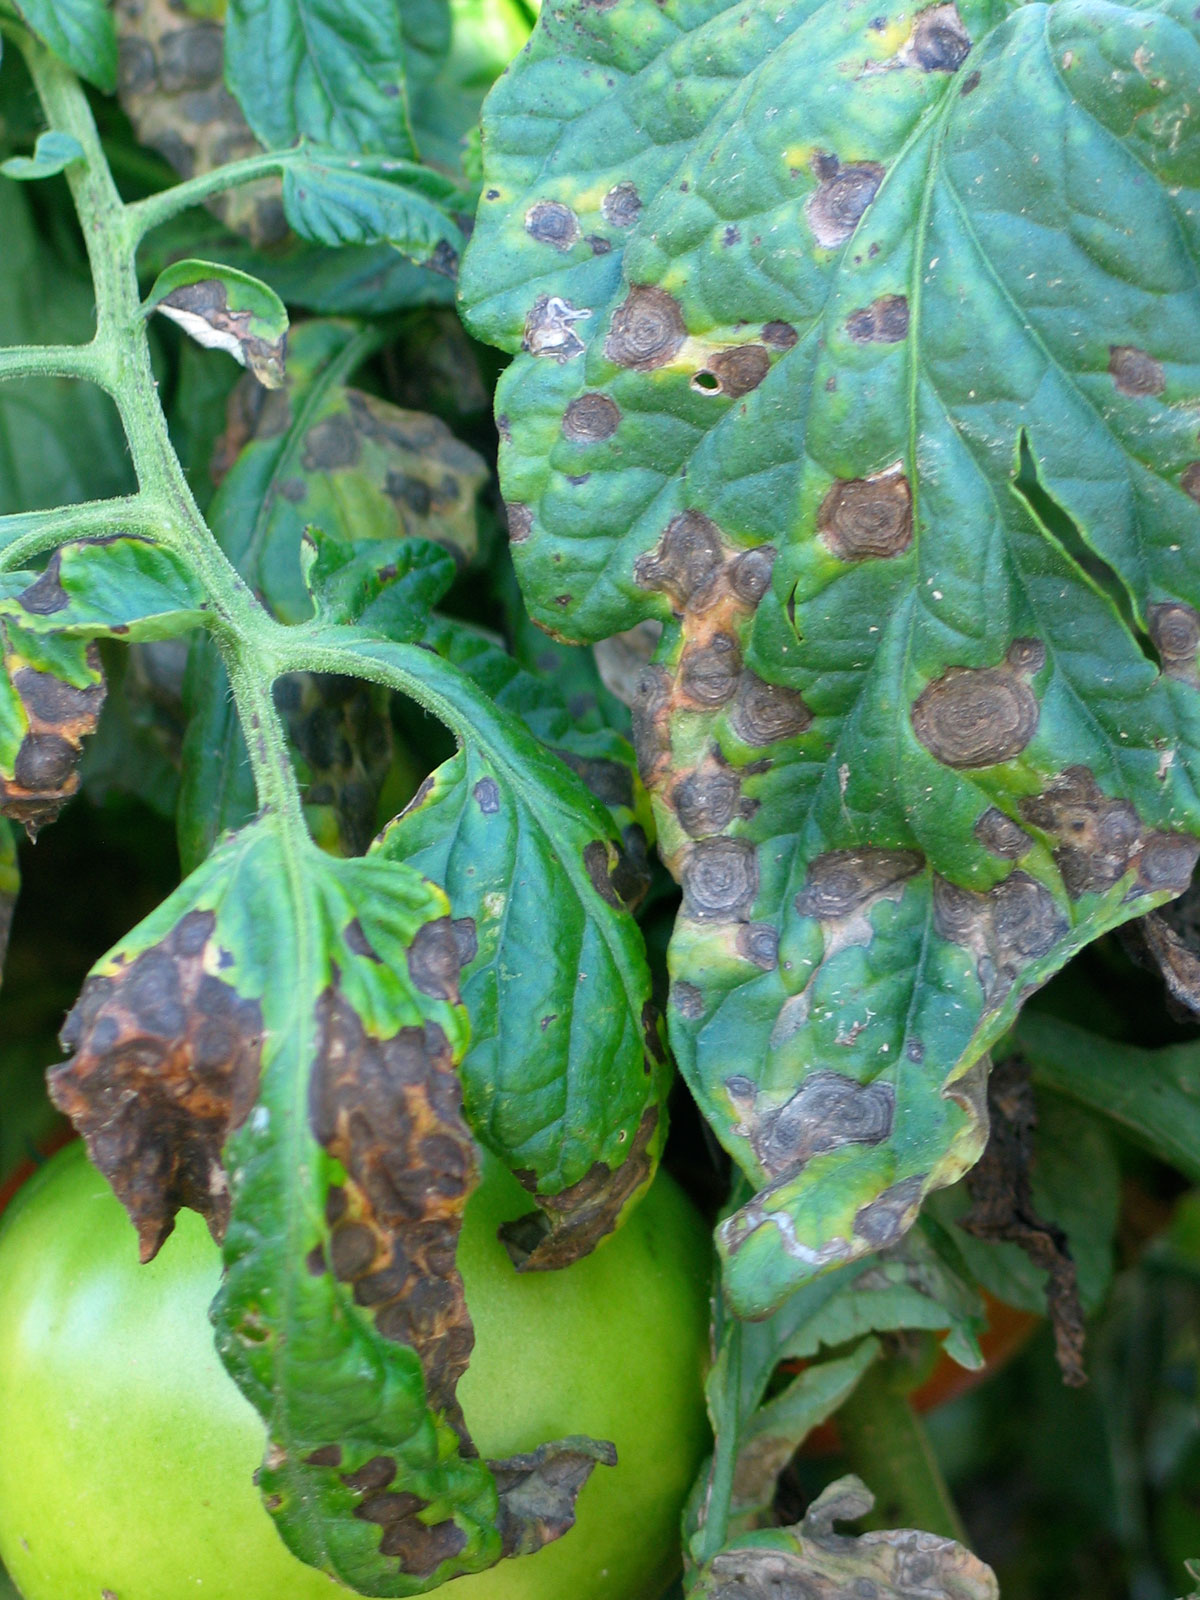
\includegraphics[height=1.8in,width=.95\linewidth,keepaspectratio]{../examples/field_second.jpg}\\
\small Label: early blight.\\Ordinary: \DemoOrdTwo.\\Strong: \DemoAugTwo.
\end{minipage}
\captionof{figure}{Two fixed legacy demonstration photographs, scored by the new seed-664 pair. They were selected during the original analysis, before the fresh-view runs, and do not estimate typical performance. Exact paths and credits appear in \code{examples/credits.csv}.}
\end{center}

\textbf{Reading the examples.} Individual corrections or regressions do not determine the main conclusion. We use all test images and all prespecified seeds for that comparison. The executed Notebook loads actual checkpoints for offline inference, checks the example hashes, and compares the predictions with the saved full-test evidence.

\textbf{What stronger evidence would require.} New independently diagnosed field leaves, especially underrepresented diseases, would address a different uncertainty from additional training seeds. Fresh sampling and three independent initializations improve the training study; they do not repair label ambiguity, related web photographs, or deployment representativeness.
\clearpage

\section{Limitations and conclusion}
\FreshConclusion\ This applies to the specified backbone, partial fine-tuning, resolution, budget, transformations, and collections. It does not establish the behavior of all augmentation strategies or a reliable field diagnostic system.

Mosaic virus still lacks validation support. Unknown leaf IDs and near-duplicates prevent a full independence guarantee. PlantDoc is an internet-collected cropped-image benchmark with ambiguous examples, not a prospective collection of independently diagnosed farm leaves. Its two spider-mite entries provide weak class evidence. Three seeds describe limited optimization variation, not variation across farms, seasons, or dataset construction.

This follow-up was designed after inspecting the original field results. Field labels never enter optimization or checkpoint selection, but the benchmark was already examined: this is exploratory follow-up evidence, not a pristine confirmatory external test. A stronger study would predefine a new target-development/test separation and evaluate on an independent field collection. Target-domain fine-tuning must use its own development subset.

\section{Reproducibility and provenance}
\code{experiment_fresh.py} executed the six new training runs. \code{results/fresh_views/} includes the frozen protocol, timestamped events, all selected weights, per-epoch histories, per-image probabilities, class metrics, and audits. \code{selection_locked.json} records all six checkpoint hashes before test scoring. \code{summarize_fresh.py} verifies paired initialization/order, budgets, checkpoint hashes, and per-seed result integrity. All six models completed eight epochs; these are independently trained weights from this delivery.

The original weights and predictions remain separate and unchanged. Their optimization history is supplied evidence. Independently reconstructing their file list and replaying both checkpoints on all 4,093 raw test images reproduced all 8,186 labels (probability differences below 0.000260). Replay confirms inference, not the original training history.

The executed Notebook expands the methods, recomputes multi-seed statistics, and loads fresh checkpoints for example inference. Its default execution does not repeat training. The package includes the source, LaTeX figures/tables, basic editable slides, environment requirements, checksums, and runnable commands. Replace Author Name(s) with actual authors before submission.

\begin{thebibliography}{9}\small
\bibitem{pv} S. P. Mohanty, D. P. Hughes, and M. Salath\'e. Using Deep Learning for Image-Based Plant Disease Detection. \emph{Frontiers in Plant Science}, 7:1419, 2016. \url{https://doi.org/10.3389/fpls.2016.01419}. Data and leaf metadata: \url{https://github.com/spMohanty/PlantVillage-Dataset}; official split lists: \url{https://huggingface.co/datasets/mohanty/PlantVillage/tree/main/splits}.
\bibitem{pd} D. Singh et al. PlantDoc: A Dataset for Visual Plant Disease Detection. \emph{CoDS-COMAD}, 2020. \url{https://doi.org/10.1145/3371158.3371196}. Cropped classification data: \url{https://github.com/pratikkayal/PlantDoc-Dataset}, CC BY 4.0.
\bibitem{mobile} A. Howard et al. Searching for MobileNetV3. \emph{ICCV}, 2019. \url{https://arxiv.org/abs/1905.02244}. Fresh runs: torchvision 0.22.1, \code{IMAGENET1K_V1}; legacy: torchvision 0.20.1 with the same ImageNet initialization.
\end{thebibliography}
\end{document}
